\chapter{МЕТОДЫ И КОМПЛЕКСЫ ОБРАБОТКИ ЕСТЕСТВЕННОГО ЯЗЫКА} \label{chapt2}

\section{Обработка Эталонных Текстов} \label{sect2_1}
В данном разделе проводится обзор обработчиков естественного языка. За основу были взяты инциденты из выгрузки систем поддержки ОАО "ICL КПО-ВС". \\
Ввиду специфики области основным языком был выбран английский язык. Был сформирован список из типичных эталонных фраз, на которых тестировались обработчики естественного языка. Фразы были выявлены путем анализа существующих отчетов об инцидентах. Примерами инцидентов являются следующие инциденты:\\
\textbf{Инцидент 1}
\textit{
User had received wrong application. User has ordered Wordfinder Business Economical for her service tag 7Q4TC3J, there is completed order in LOT with number ITCOORD-18125. However she received wrong version, she received Wordfinder Tehcnical instead of Business Economical. Please assist.
}\\
\textbf{Инцидент 2}
\textit{
Laptop – user has almost full C:\ but when he looks in the properties of the files and folders on C:\ they are only 40GB and he has a 55GB drive.
}\\
\textbf{Инцидент 3}
\textit{
User cannot find Produkt Manageron start menu. Please reinstall. 
}\\
\textbf{Инцидент 4}
\textit{
User needs to have pdf 995 re-installed please.
}\\

Во время анализа были использованы следующие обработчики естественного языка:
\begin {enumerate}
	\item{Open NLP}\cite{OpenNLP}
	\item{RelEx}\cite{OpenCogRelex}
	\item{StanfordParser}\cite{StanfordParser}
\end {enumerate}

Результат работы вычислялся при помощи метрик, представленных в Таблице\ref{Metrics}. 

\begin{table} [htbp]
  \centering
  \parbox{15cm}{\caption{Таблица метрик}\label{Metrics}}
%  \begin{center}
  \begin{tabular}{| p{5cm} ||p{5cm}|| p{5cm} |}
  \hline
  \hline
Метрика & Описание & Формула \\
  \hline
  \hline
Аккуратность	& Понимание текста обработчиком & 
$$ 
Ac=\frac{1-x}{y}
$$ где x- количество нераспознанныx слов, y количество распознанных \\
 \hline
Успешно обработанные	& Успешно обработанные инциденты & 
$$ 
P=\frac{x}{100}
$$ где x успешно обработанные \\
 \hline
Не успешно обработанные	& Неуспешно обработанные инциденты & 
$$ 
N=\frac{y}{100}
$$ где y неуспешные инциденты \\
 \hline
Результативность	& Общая результативность обработчика & 
$$ 
R=\frac{P}{N}
$$  \\
  \hline
  Общий бал	& Общая оценка обработчика & 
$$ 
T=Ac+R
$$  \\
  \hline
  \hline
  \end{tabular}
%  \end{center}
\end{table}

Результаты приведены на сводной диаграмме Рисунок \ref{img:ParserComp}

\begin{figure} [h] 
  \center
  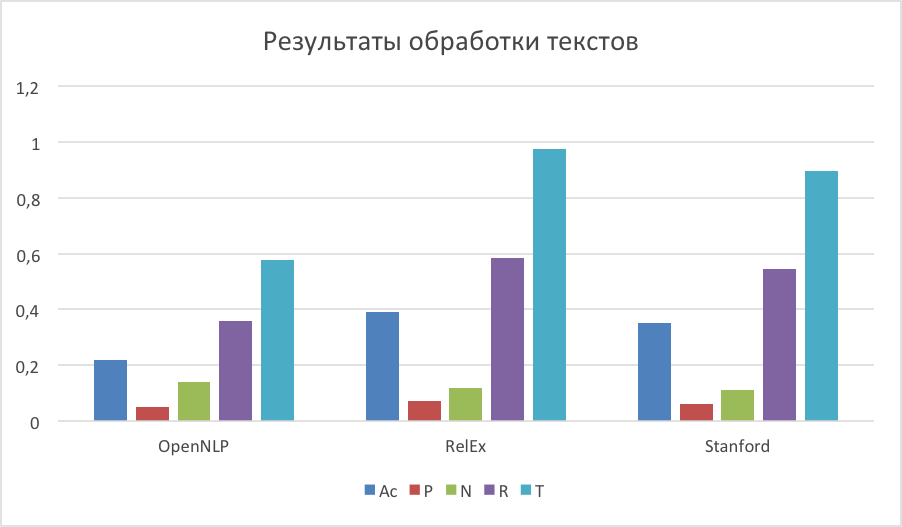
\includegraphics [scale=1.0] {ParserCompare}
  \caption{Результаты обработки текстов} 
  \label{img:ParserComp}  
\end{figure}

Из диаграммы видно, что наилучшее результаты показывает обработчик RelEx\cite{OpenCogRelex}. После анализа необработанных инцидентов было выявлено нескольких проблем у всех обработчиков:
\begin{enumerate}
	\item Невозможности корректировки простых грамматических ошибок, связанных с пропущенными пробелами или неверным форматированием. Ошибки первого типа.
	\item Ошибки неверной интерпретации слов в предложении. Например, слово please интерпретировалось как глагол, хотя является по смыслу «формой вежливости». Ошибки второго типа.
\end{enumerate}	

	
 
%\newpage
%============================================================================================================================
\section{Обработка текстов с ошибками} \label{sect2_2}

По результатам прошлого раздела было решено выбрать в качестве обработчика естественного языка RelEx, но были выявлены некоторые проблемы. Было принято решение исправить данные проблемы при помощи предварительной обработки текста. Предварительная обработка текста была разбита на несколько фаз:
\begin{enumerate}
	\item Комплексная корректировка ошибок
	\item Обработка при помощи внутренней базы знаний
\end{enumerate}
Для того, чтобы избавится от орфографический, синтаксических ошибок используется составной корректировщик. Данный компонент имеет модульную структуру и применяет корректировку последовательно.
\begin{figure} [h] 
  \center
  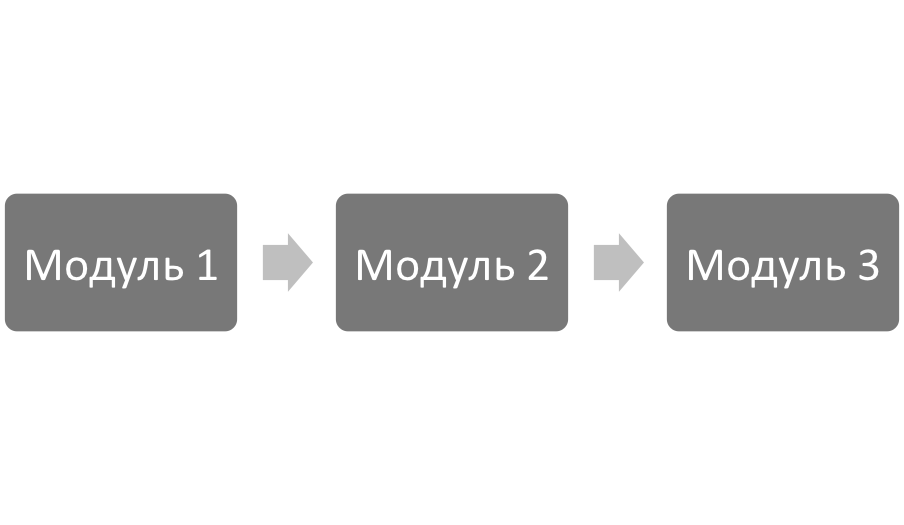
\includegraphics [scale=1.0] {SpellCorrector}
  \caption{Архитектура предварительной обработки текста} 
  \label{img:SpellCorrector}  
\end{figure}

Для данного компонента были написаны модули корректировки:
\begin{itemize}
	\item Google API
	\item After The Deadline
\end{itemize}
Таким образом удалось исправить большинство ошибок, связанный с синтаксисом, грамматикой, орфографии. Также удалось исправить ошибки неверного написания: лишних пробелов, пропущенных запятых, пропущенных точек.
По-прежнему остается проблема обработки неверной интерпретации слов в тексте. \\

Для корректировка ошибок второго типа был использовано инъекция в работу обработчика RelEx. В ввиду OpenSource природы проекта, модульности был подменен модуль извлечения и обработки слов в предложения. Стандартный процесс обработки был разбит на «предобработку» и «обработку». Стадия «обработки» включала в себя алгоритм работы такой же как был до этого в модули, на стадии «предобработки» управление передается модулю основному приложению, который проверяет данное слово на предмет его вхождения во внутреннюю Базу Знаний и если таковое имеется, то приложение передает соответствующие корректировки в модуль

%\newpage
%============================================================================================================================
\section{Сравнение средств обработки русского и английского языка} \label{sect2_3}
Средства обработки естественного языка принято относить в большому классу средств NLP – Natural Language Processing. Для английского языка существует множество открытых средств обработки естественного языка, для русского языка найти их гораздо сложнее. Рассмотрим архитектуру средств обработки естественного языка на примере OpenCog RelEx. \\
OpenCog RelEx использует результаты обработки Link Grammar \cite{linkgrammar}. Link Grammar поддерживает множество языков: английский, русский, турецкий, немецкий и т.д.  RelEx использует вывод LG и преобразует его в формат связей.
\textbf{Пример 1}. User is unable to start KDP web, please reinstall Java.\\
\textbf{Результат} 
\begin{verbatim}
		_obj(start, KBP)
pos(start, verb)
inflection-TAG(start, .v)
tense(start, present)
pos([web], WORD)
noun_number(KBP, singular)
definite-FLAG(KBP, T)
pos(KBP, noun)
_advmod(reinstall, please)
pos(reinstall, verb)
inflection-TAG(reinstall, .v)
tense(reinstall, present)
pos(please, adv)
inflection-TAG(please, .e)
noun_number(Java, singular)
definite-FLAG(Java, T)
pos(Java, noun)
pos(., punctuation)
_obj(,, Java)
pos(,, verb)
tense(,, infinitive)
HYP(,, T)
_to-do(unable, ,)
pos(unable, adj)
inflection-TAG(unable, .a)
tense(unable, present)
pos(to, prep)
inflection-TAG(to, .r)
pos(be, verb)
inflection-TAG(be, .v)
_predadj(User, unable)
noun_number(User, singular)
definite-FLAG(User, T)
pos(User, noun)

\end{verbatim}



Возьмем разбор слова start. В результате мы получаем несколько отношений:
\begin{itemize}
	\item pos(start, verb) - start глагол
	\item tense(start, present) - время настоящее
	\item inflection-TAG(start, .v) -  метод обозначения на схеме (индекс)
\end{itemize}

На их основе можно формализовать приложение на естественном языке. Остальные парсера пока не поддерживают русский язык. Существуют открытые проекты, но они еще недостаточно развиты.
\section{Вывод по главе} \label{sect2_4}
В данный главе был выполнен основной анализ обработчиков естественного языка. Ввиду развитости и доступности было решено использовать OpenCog RelEx.
\clearpage
